\documentclass[11pt]{article}
\usepackage{preamble}
\usepackage{amssymb}

\newcommand{\IconCheck}{[CHECK]}
\newcommand{\IconMic}{[MIC]}
\newcommand{\IconClipboard}{[CLIPBOARD]}

\newcommand{\phasetag}[1]{%
  {\small\itshape Tag: #1\par}
}

\newcommand{\phaseitems}[1]{%
  \begin{itemize}[leftmargin=1.5em,itemsep=2pt,topsep=2pt]
  #1
  \end{itemize}%
}

\newcommand{\teacheranswerbox}[2]{%
  \begin{callout}{#1}{calloutgreen}
  #2
  \end{callout}
}

\begin{document}

\packetheading{Lesson 6-4 \(\cdot\) Quick \(\cdot\) Teacher Edition}{Logarithmic Functions + DOK-3 Sales Revenue Inverse (Item 28)}

\sectionbanner{OBJECTIVES}
{\small
\renewcommand{\arraystretch}{1.25}
\noindent\begin{tabular}{|p{1.8in}|p{4.8in}|}
\hline
\textbf{Math Objective} & Graph logarithmic functions, identify key features (asymptote, domain, range, intercepts), and find equations of inverses of exponential and logarithmic functions. \\ \hline
\textbf{Language Objective} & Describe how transforming a log function shifts its asymptote and key points; explain why the inverse of a log is an exponential. \\ \hline
\textbf{Essential Understanding} & Log and exponential functions are inverses --- swap \(x\) and \(y\), solve. The asymptote of a log is the y-axis mirror of an exp function's horizontal asymptote. \\ \hline
\end{tabular}
}

\sectionbanner{TOPIC GOALS / ESSENTIAL QUESTION / MATERIALS}
{\small
\renewcommand{\arraystretch}{1.25}
\noindent\begin{tabular}{|p{1.8in}|p{4.8in}|}
\hline
\textbf{Topic Goals} & Fluency with graphing log functions and finding inverses; apply to the Sales Revenue DOK-3 task (Item 28 rehearsal for Form B model-then-invert structure). \\ \hline
\textbf{Essential Question} & How do the graphs of logarithmic and exponential functions relate, and how do we find one from the other? \\ \hline
\textbf{Materials} & Student packet, pencil, calculator. Rules card: \(\log_b 1 = 0\); \(\log_b b = 1\); \(y = \log_b x\) has VA at \(x = 0\); \(y = \log_b(x - h) + k\) has VA at \(x = h\); inverse of \(y = a \cdot b^x\) is \(y = \log_b(x/a)\); inverse of \(y = \log_b(x - h) + k\) is \(y = b^{(x-k)} + h\). \\ \hline
\end{tabular}
}

\begin{callout}{\IconPin\ PRE-FLIGHT --- SINGLE-PERIOD COMPRESSED LESSON + DOK-3 CAPSTONE}{calloutpink}
This is a single-period quick treatment of Lesson 6-4. ONE example modeled in Launch (Ex 3B: inverse of \(g(x)=\log_7(x+5)\) + composition verification). Contrast with Ex 3A (inverse of exponential) in 90 sec only --- same swap-and-solve process, direction reversed. Release to Explore at minute 15.\\
DOK-3 driver: Practice \#28 (\(R = 12\log(a+1)+25\)). Students (a) find the inverse function \(a = 10^{\frac{R-25}{12}} - 1\), (b) judge which form is easier for specific \(R\) values. Real Savvas values from SE source.\\
Pace: \IconStar\ q28 (10 min) \(\rightarrow\) q21 (4 min) \(\rightarrow\) q24 (4 min) \(\rightarrow\) q13 (4 min) \(\rightarrow\) q9 (3 min). \(\sim\)25 min total Explore.\\
45-min Wed F variant: cut q9. Never cut q28.\\
Assessment alignment: q21\(\rightarrow\)Form B Q7, q24\(\rightarrow\)Q12, q13\(\rightarrow\)Q11, q9\(\rightarrow\)Q9/Q10, q28\(\rightarrow\)DOK-3 rehearsal.
\end{callout}

\phasetag{bridge to log inverses launch}
\frameworkphaseheader{Do Now}{1--2}{7}{%
\phaseitems{
  \item Hand out at door.
  \item Circulate 4 min.
  \item Cold-call on q31: ask which transformation shifts the VA.
  \item Pull sheets at minute 7.
}%
}{%
\phaseitems{
  \item q31: translation multi-select for \(h(x)=\ln(x+2)-1\).
  \item q5: graph \(y=\log_4 x\) with all key features.
  \item q32: find inverse of \(f(x)=5^{x+1}\) (SAT/ACT).
}%
}{%
\phaseitems{
  \item q31: how does \((x+2)\) inside the log change the VA?
  \item q5: domain? VA? x-intercept? End behavior as \(x \rightarrow 0^+\) and \(x \rightarrow \infty\)?
  \item q32: undo \(5^x\) using log base 5 --- what is the inverse operation?
}%
}{Solo teacher: circulate silently. No hints on q32.}

\bankitem{Do Now 1 --- Translation identification: \(h(x)=\ln(x+2)-1\)}{%
The logarithmic function \(g(x)=\ln x\) is transformed to \(h(x)=\ln(x+2)-1\). Which of the following are true? Select all that apply.

\begin{itemize}[leftmargin=1.5em,itemsep=4pt,topsep=5pt]
  \item[\(\square\)] \(g(x)\) is translated 2 units upward.
  \item[\(\square\)] \(g(x)\) is translated 2 units to the right.
  \item[\(\square\)] \(g(x)\) is translated 2 units to the left.
  \item[\(\square\)] \(g(x)\) is translated 1 unit downward.
  \item[\(\square\)] \(g(x)\) is translated 1 unit to the left.
  \item[\(\square\)] The vertical asymptote shifts 2 units to the left.
  \item[\(\square\)] The vertical asymptote shifts 2 units to the right.
\end{itemize}
}{}

\teacheranswerbox{\IconCheck\ ANSWER KEY}{%
\textbf{Answer key (from source):} \(g(x)\) is translated 2 units to the left; \(g(x)\) is translated 1 unit downward; The vertical asymptote shifts 2 units to the left.
}

\bankitem{Do Now 2 --- Graph \(y=\log_4 x\); state key features}{%
Graph the function \(y = \log_4 x\) and identify the domain and range. List any intercepts or asymptotes. Describe the end behavior.
}{}

\teacheranswerbox{\IconCheck\ ANSWER KEY}{%
\begin{center}
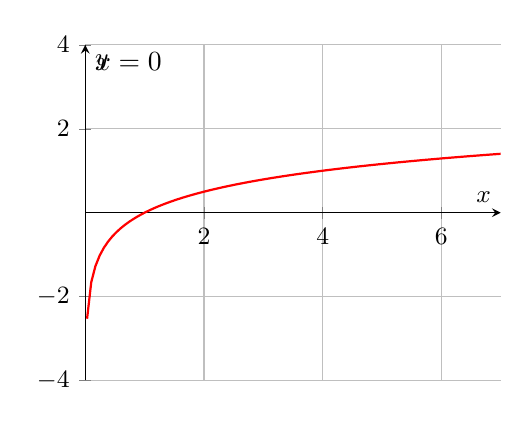
\begin{tikzpicture}
\begin{axis}[
  width=2.7in,
  height=2.3in,
  axis lines=middle,
  xmin=0,
  xmax=7,
  ymin=-4,
  ymax=4,
  xtick={0,2,4,6},
  ytick={-4,-2,0,2,4},
  xlabel={$x$},
  ylabel={$y$},
  grid=both,
  tick label style={font=\small},
  label style={font=\small}
]
\addplot[red, thick, domain=0.03:7, samples=100] {ln(x)/ln(4)};
\draw[dashed] (axis cs:0,-4) -- (axis cs:0,4) node[pos=0.95,right] {$x=0$};
\end{axis}
\end{tikzpicture}
\end{center}
\textbf{Answer key (from source):} Domain: \(\{x \mid x>0\}\); range: all real numbers; \(x\)-intercept: 1; asymptote: \(y\)-axis; end behavior: As \(x \rightarrow 0\), \(y \rightarrow -\infty\). As \(x \rightarrow \infty\), \(y \rightarrow \infty\).
}

\bankitem{Do Now 3 --- SAT/ACT: inverse of \(f(x)=5^{x+1}\)}{%
\textbf{SAT/ACT} The graph shows the exponential function \(f(x) = 5^{x+1}\). Which of the following functions represents its inverse, \(f^{-1}(x)\)?

\begin{center}
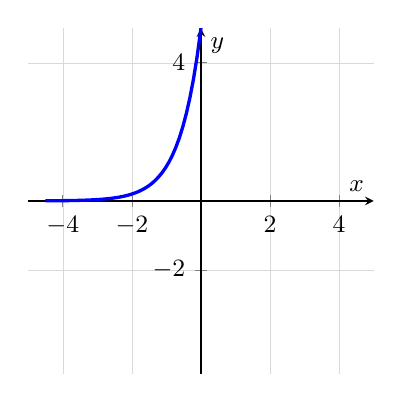
\begin{tikzpicture}
\begin{axis}[
  width=2.35in,
  height=2.35in,
  axis lines=middle,
  xmin=-4.5,
  xmax=4.5,
  ymin=-4.5,
  ymax=4.5,
  xtick={-4,-2,2,4},
  ytick={-2,4},
  grid=both,
  grid style={line width=.1pt, draw=gray!30},
  enlargelimits={abs=0.5},
  xlabel={$x$},
  ylabel={$y$},
  tick label style={font=\small},
  label style={font=\small}
]
\addplot[domain=-4.5:0.5, samples=50, blue, line width=1.2pt] {5^(x+1)};
\end{axis}
\end{tikzpicture}
\end{center}

\begin{center}
\begin{tabular}{ll}
\textcircled{A} \(f^{-1}(x) = 1 + \log_5 x\) & \textcircled{B} \(f^{-1}(x) = \log_5 x - 1\) \\
\textcircled{C} \(f^{-1}(x) = \log_5 (x - 1)\) & \textcircled{D} \(f^{-1}(x) = \log_5 (x + 1)\)
\end{tabular}
\end{center}
}{}

\teacheranswerbox{\IconCheck\ ANSWER KEY}{%
\textbf{Answer key:} \textcircled{B} \(f^{-1}(x) = \log_5 x - 1\). Swap \(x\) and \(y\): \(x = 5^{y+1}\), so \(y+1 = \log_5 x\) and \(y = \log_5 x - 1\).
}

\begin{callout}{\IconCheck\ ANSWER KEY}{calloutgreen}
Answer key (from source): \(g(x)\) is translated 2 units to the left; \(g(x)\) is translated 1 unit downward; The vertical asymptote shifts 2 units to the left.\\
(verify before class)\\
(verify before class)
\end{callout}

\phasetag{teacher models Ex 3B (inverse of log) + 90s Ex 3A contrast}
\frameworkphaseheader{Launch}{2}{8}{%
\phaseitems{
  \item Project Ex 3B. Think aloud: \(g(x) = \log_7(x+5)\). Step 1: swap \(x\) and \(y\). Step 2: write \(7^x = y+5\). Step 3: solve --- \(y = 7^x - 5\).
  \item ``Now verify with composition: \(g(g^{-1}(x)) = \log_7((7^x-5)+5) = \log_7(7^x) = x.\) \(\checkmark\)''
  \item 90-sec contrast: Ex 3A (inverse of exponential, e.g. \(y = 3 \cdot 5^x\)). ``Swap \(x\) and \(y\) \(\rightarrow\) \(x = 3 \cdot 5^y\) \(\rightarrow\) \(x/3 = 5^y\) \(\rightarrow\) \(y = \log_5(x/3)\). Same swap-and-solve.''
  \item Flag the Rules card --- students copy VA shift rule and inverse rules into margin.
  \item 30-sec pause: partner repeats the inverse steps in their own words.
  \item Do NOT solve Explore items --- release at minute 15.
}%
}{%
\phaseitems{
  \item Watch Ex 3B silently. Note swap-then-solve sequence.
  \item Copy composition verification step.
  \item During 90-sec contrast: note that inverting an exponential gives a log, and inverting a log gives an exponential.
  \item Copy Rules card VA and inverse rules into margin.
}%
}{%
\phaseitems{
  \item In \(g(x)=\log_7(x+5)\), what is the domain? VA? (\(x=-5\))
  \item After swapping \(x\) and \(y\), how do we isolate \(y\) when \(7^x = y+5\)?
  \item What is \(g^{-1}(x)\)? What is its domain? (\(x \in \mathbb{R}\))
  \item Why does the VA of \(g\) become the HA of \(g^{-1}\)?
}%
}{Project Ex 3B. Model composition check. 90-sec Ex 3A contrast. Release promptly at minute 15.}

\bankitem{Example 3B}{%
\textbf{Inverses of Exponential and Logarithmic Functions}

What is the equation of the inverse of the functions?

\textbf{A. \(f(x) = 10^{x+1}\)}
\begin{align*}
y &= 10^{x+1} \\
x &= 10^{y+1} \quad \text{(Rewrite the function as \(y=\), interchange \(x\) and \(y\), and solve for \(y\).)} \\
y + 1 &= \log x \\
y &= \log x - 1
\end{align*}
The equation of the inverse of \(f(x) = 10^{x+1}\) is \(f^{-1}(x) = \log x - 1\).

Verify by function composition.
\begin{align*}
f(f^{-1}(x)) &= 10^{(\log x - 1) + 1} & f^{-1}(f(x)) &= \log 10^{x+1} - 1 \\
&= 10^{\log x} & &= x + 1 - 1 \\
&= x & &= x
\end{align*}

\begin{center}
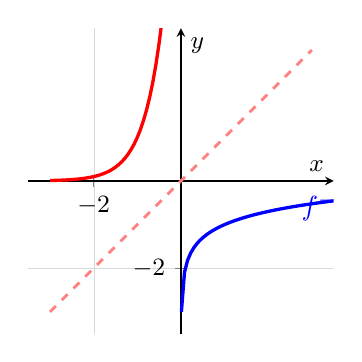
\begin{tikzpicture}
\begin{axis}[
  width=2.15in,
  height=2.15in,
  axis lines=middle,
  xmin=-3,
  xmax=3,
  ymin=-3,
  ymax=3,
  xtick={-2},
  ytick={-2},
  grid=both,
  grid style={line width=.1pt, draw=gray!30},
  enlargelimits={abs=0.5},
  xlabel={$x$},
  ylabel={$y$},
  tick label style={font=\small},
  label style={font=\small}
]
\addplot[domain=-3:3, samples=20, dashed, red!50!white, line width=1pt] {x};
\addplot[domain=-3:0.5, samples=50, red, line width=1.2pt] {10^(x+1)} node[pos=0.8, left] {$f$};
\addplot[domain=0.01:3.5, samples=50, blue, line width=1.2pt] {log10(x)-1} node[pos=0.8, right] {$f^{-1}$};
\end{axis}
\end{tikzpicture}
\end{center}

\begin{callout}{CONCEPTUAL UNDERSTANDING / LOOK FOR RELATIONSHIPS}{calloutyellow}
\(f(x)\) is a translation of the parent function \(y = 10^x\) one unit left. \(f^{-1}(x)\) is a translation of the parent function \(y = \log x\) one unit down. Graphical translations of a function and its inverse are directly related. Explain.
\end{callout}

\textbf{B. \(g(x) = \log_7(x + 5)\)}
\begin{align*}
y &= \log_7(x + 5) \quad \text{(Rewrite as \(y=\).)} \\
x &= \log_7(y + 5) \\
y + 5 &= 7^x \\
y &= 7^x - 5
\end{align*}
The equation of the inverse of \(g(x) = \log_7(x + 5)\) is \(g^{-1}(x) = 7^x - 5\).

Verify by function composition.
\begin{align*}
g(g^{-1}(x)) &= \log_7(7^x - 5 + 5) & g^{-1}(g(x)) &= 7^{\log_7(x + 5)} - 5 \\
&= \log_7 7^x & &= x + 5 - 5 \\
&= x & &= x
\end{align*}

\begin{center}
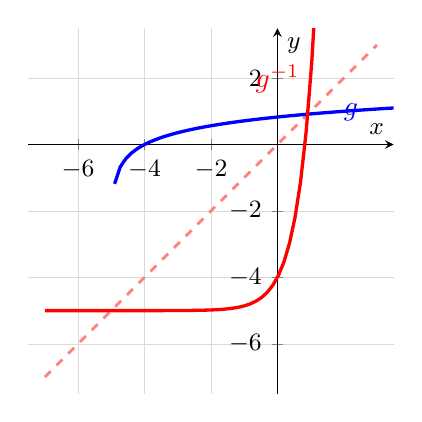
\begin{tikzpicture}
\begin{axis}[
  width=2.45in,
  height=2.45in,
  axis lines=middle,
  xmin=-7,
  xmax=3,
  ymin=-7,
  ymax=3,
  xtick={-6,-4,-2},
  ytick={-6,-4,-2,2},
  grid=both,
  grid style={line width=.1pt, draw=gray!30},
  enlargelimits={abs=0.5},
  xlabel={$x$},
  ylabel={$y$},
  tick label style={font=\small},
  label style={font=\small}
]
\addplot[domain=-7:3, samples=20, dashed, red!50!white, line width=1pt] {x};
\addplot[domain=-4.9:3.5, samples=50, blue, line width=1.2pt] {ln(x+5)/ln(7)} node[pos=0.8, right] {$g$};
\addplot[domain=-7:1.2, samples=50, red, line width=1.2pt] {7^x - 5} node[pos=0.8, left] {$g^{-1}$};
\end{axis}
\end{tikzpicture}
\end{center}
}{}

\teacheranswerbox{\IconCheck\ ANSWER KEY}{%
The equation of the inverse of \(f(x) = 10^{x+1}\) is \(f^{-1}(x) = \log x - 1\).\\
The equation of the inverse of \(g(x) = \log_7(x + 5)\) is \(g^{-1}(x) = 7^x - 5\).
}

\begin{callout}{\IconMic\ TEACHER SCRIPT}{calloutblue}
1. ``Watch me find the inverse of a LOG function.''\\
2. ``Step 1: replace \(g(x)\) with \(y\). Step 2: swap \(x\) and \(y\).''\\
3. ``Step 3: rewrite in exponential form --- \(7^x = y+5\).''\\
4. ``Step 4: solve for \(y\) --- \(y = 7^x - 5\). That's \(g^{-1}(x)\).''\\
5. ``Composition check: \(g(g^{-1}(x)) = \log_7(7^x-5+5) = x.\) \(\checkmark\)''\\
6. ``Now 90 seconds: Ex 3A --- inverting an exponential gives a log. Same swap-and-solve.''\\
7. Release to Explore.
\end{callout}

\phasetag{TPS + DOK-3 driver}
\frameworkphaseheader{Explore}{2--3}{25}{%
\phaseitems{
  \item 4 laps across 25 min.
  \item Lap 1 (10 min): \IconStar\ q28 DOK-3. Press pairs on inverse setup and form comparison. DO NOT give the inverse formula --- redirect with `what does it mean to undo \(R\)?'
  \item Lap 2 (4 min): q21. Press notation: what is the inverse of \(5^{x-3}\)?
  \item Lap 3 (4 min): q24. Press: inverse of \(\log_2(8x)\) --- watch for domain.
  \item Lap 4 (4 min): q13. Press: how does the horizontal shift move the VA?
  \item Lap 5 (3 min): q9. Are graphs inverses? Key test: reflective symmetry over \(y=x\).
  \item 45-min Wed F: skip q9.
}%
}{%
\phaseitems{
  \item 5 items in order: \IconStar\ q28 \(\rightarrow\) q21 \(\rightarrow\) q24 \(\rightarrow\) q13 \(\rightarrow\) q9.
  \item For q28: BEFORE computing, write down \(R = 12\log(a+1)+25\) and plan how to isolate \(a\).
  \item For q28 part 2: decide which form (original or inverse) is easier for \(R = 49\) and \(R = 61\). Write a justification sentence.
}%
}{%
\phaseitems{
  \item q28: how do you undo +25 first? Then undo \(\times 12\)?
  \item q28: after \((R-25)/12 = \log(a+1)\), what is the next step?
  \item q28: for \(R=49\), would you use \(R=12\log(a+1)+25\) or \(a=10^{\frac{R-25}{12}}-1\)? Why?
  \item q21: identify base and exponent --- what is the log that undoes \(5^x\)?
  \item q24: inverse of \(\log_2(8x)\) --- swap \(x\) and \(y\) first. Then rewrite.
  \item q13: find the VA of the translated log from the graph.
  \item q9: if two graphs are inverses, what visual test do they pass?
}%
}{Solo teacher: 4 laps. On q28, press the judgment step (which form and why) --- that is the DOK-3 performance criterion.}

\begin{callout}{\IconSpeak\ CHAIN 1 CALLBACK --- Revenue Inverse (PEAK, 5 priors)}{calloutpeach}
\textit{When to say:} Before students start Practice \#28.

\smallskip
``We've done this five times now: Storage Box, wavelength, cylinder, Richter, and today revenue. Every time: a model, a constraint, a hidden input we want to recover. Today's twist: the original model is \textbf{exponential}, so to invert it we need a \textbf{logarithm}. That's why we spent yesterday on logs. A log isn't a new topic --- it's the specific tool that lets us invert an exponential model. Same job we've been doing all year, new lock, new key.''

\smallskip
\textit{Note:} q33 (Telescope Magnitude, fast-finisher) is the Chain 1 micro-callback: ``Another physical formula, another extraction. At this point you should be able to see the shape from a mile away --- constraint plus inversion.''
\end{callout}

\bankitem{Practice \#28 \IconStar\ DOK-3 SALES REVENUE INVERSE --- Form B model-then-invert rehearsal}{%
A company uses this function to relate sales revenue, \(R\), and advertising costs, \(a\). What is the equation of the inverse of the equation? Which equation would be easier to use to find a value of \(a\) for a particular value of \(R\)?

\begin{center}
\begin{tikzpicture}[>=stealth, font=\small, line width=0.9pt]
\node[draw, rounded corners, fill=frameshade, minimum width=1.95in, minimum height=0.85in, align=center] (rev) at (0,0) {\textbf{Sales Revenue, \(R\)}\\\vspace{2pt}o\hspace{4pt}o\hspace{4pt}o};
\node[draw, rounded corners, fill=frameshade, minimum width=2.1in, minimum height=0.85in, align=center] (ads) at (5.0,0) {\textbf{Advertising Costs, \(a\)}\\\vspace{2pt}\fbox{\strut ADS}\hspace{0.4em}\fbox{\strut PHONE}};
\draw[->, tealheader] (ads.west) -- node[above, align=center] {\(R = 12\log(a+1)+25\)} (rev.east);
\end{tikzpicture}
\end{center}
}{}

\begin{callout}{\IconStar\ DOK-3 SALES REVENUE --- Practice \#28}{calloutpink}
Students must (a) isolate \(a\) from \(R = 12\log(a+1)+25\), yielding \(a = 10^{\frac{R-25}{12}} - 1\), (b) judge which form is easier for specific \(R\) values.\\
Key criteria: (1) correct algebraic isolation steps shown, (2) inverse formula correct (base 10, not natural log), (3) justification for form preference cites a specific computation.\\
Assessment alignment: DOK-3 rehearsal for Form B model-then-invert structure
\end{callout}

\teacheranswerbox{\IconCheck\ ANSWER / ANTICIPATED TALK}{%
The inverse of the formula is \(a=10^{\frac{R-25}{12}}-1\). It would be easier to use the inverse to find \(a\) when \(R\) is known.\\
Assessment alignment: DOK-3 rehearsal for Form B model-then-invert structure
}

\bankitem{Practice \#21 --- Inverse of exponential \(5^{x-3}\) [Form B Q7 rehearsal]}{%
Find the equation of the inverse of each function. \(f(x)=5^{x-3}\).
}{}

\teacheranswerbox{\IconCheck\ ANSWER / ANTICIPATED TALK}{%
Answer key (from source): \(f^{-1}(x)=\log_5 x+3\)\\
Assessment alignment: Form B Q7: inverse of \(5^{(x-3)}\)
}

\bankitem{Practice \#24 --- Inverse of \(\log_2(8x)\), token drag [Form B Q12 rehearsal]}{%
Find the equation of the inverse of each function. \(f(x)=\log_2(8x)\).
}{}

\teacheranswerbox{\IconCheck\ ANSWER / ANTICIPATED TALK}{%
Answer key (from source): \(f^{-1}(x)=\frac{2^x}{8}\)\\
Assessment alignment: Form B Q12: inverse of \(\log_2(8x)\), token drag
}

\bankitem{Practice \#13 --- Asymptote of translated log from graph [Form B Q11 rehearsal]}{%
\textbf{Use Structure} The graph shows a transformation of the parent graph \(f(x)=\log_3 x\). Write an equation for the graph.

\begin{center}
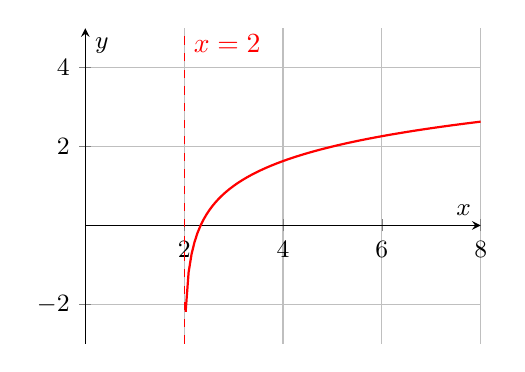
\begin{tikzpicture}
\begin{axis}[
  width=2.6in,
  height=2.2in,
  axis lines=middle,
  xmin=0,
  xmax=8,
  ymin=-3,
  ymax=5,
  xtick={0,2,4,6,8},
  ytick={-2,0,2,4},
  xlabel={$x$},
  ylabel={$y$},
  grid=both,
  tick label style={font=\small},
  label style={font=\small}
]
\addplot[red, thick, domain=2.03:8, samples=100] {ln(x-2)/ln(3)+1};
\draw[red,dashed] (axis cs:2,-3) -- (axis cs:2,5) node[pos=0.95,right] {$x=2$};
\end{axis}
\end{tikzpicture}
\end{center}
}{}

\teacheranswerbox{\IconCheck\ ANSWER / ANTICIPATED TALK}{%
Answer key (from source): \(g(x)=\log_3(x-2)+1\)\\
Assessment alignment: Form B Q11: asymptote of translated log from graph
}

\bankitem{Practice \#9 --- Are graphs inverses? Inverse from graph [Form B Q9/Q10 rehearsal]}{%
\textbf{Look for Relationships} Are the logarithmic and exponential functions shown inverses of each other? Explain.

\begin{center}
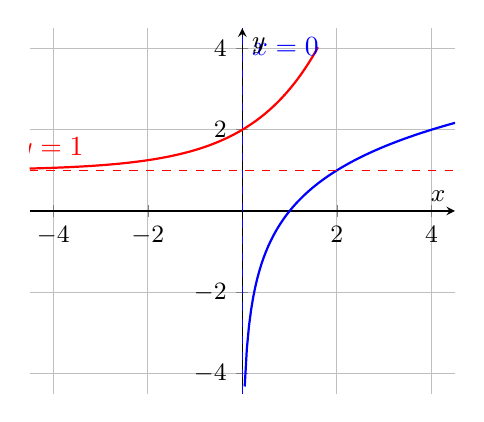
\begin{tikzpicture}
\begin{axis}[
  width=2.75in,
  height=2.45in,
  axis lines=middle,
  xmin=-4.5,
  xmax=4.5,
  ymin=-4.5,
  ymax=4.5,
  xtick={-4,-2,0,2,4},
  ytick={-4,-2,0,2,4},
  xlabel={$x$},
  ylabel={$y$},
  grid=both,
  tick label style={font=\small},
  label style={font=\small}
]
\addplot[red, thick, domain=-4.5:1.6, samples=100] {2^x+1};
\addplot[blue, thick, domain=0.05:4.5, samples=100] {ln(x)/ln(2)};
\draw[blue,dashed] (axis cs:0,-4.5) -- (axis cs:0,4.5) node[pos=0.95,right] {$x=0$};
\draw[red,dashed] (axis cs:-4.5,1) -- (axis cs:4.5,1) node[pos=0.05,above] {$y=1$};
\end{axis}
\end{tikzpicture}
\end{center}
}{}

\teacheranswerbox{\IconCheck\ ANSWER / ANTICIPATED TALK}{%
Answer key (from source): No; The \(x\)-intercept of the blue function is not equal to the \(y\)-intercept of the red function.\\
Assessment alignment: Form B Q9/Q10: are graphs inverses; inverse from graph
}

\phasetag{academic conversation + 6-5 bridge}
\frameworkphaseheader{Share / Summary}{2}{5}{%
\phaseitems{
  \item Cold-call 1 pair to present q28 solution and form-choice justification.
  \item Class signals thumbs. Write \(a = 10^{\frac{R-25}{12}} - 1\) on board.
  \item 6-5 bridge: ``Log properties (product/quotient/power rules) will let you expand and condense log expressions --- making inverses and equations faster.''
}%
}{%
\phaseitems{
  \item Presenting pair: read inverse formula and cite which form is easier for \(R=49\) and \(R=61\).
  \item Rest of class: signal thumbs and write bridge note in margin.
}%
}{%
\phaseitems{
  \item How did you isolate \(a\) from \(R = 12\log(a+1)+25\)?
  \item For \(R=49\), which form is computationally easier? Why?
}%
}{Cold-call a pair that struggled on the judgment step --- hold them accountable to citing a computation, not just a preference.}

\phasetag{inverse + asymptote (not graded)}
\frameworkphaseheader{Exit Ticket}{1--2}{5}{%
\phaseitems{
  \item Collect at door.
  \item Scan: (1) Did students swap \(x/y\) correctly? (2) Did students solve for \(y\) in exponential form? (3) Did they state VA of \(f\) as \(x=2\) and HA of \(f^{-1}\) as \(y=2\)?
}%
}{%
\phaseitems{
  \item Two-part custom exit: find inverse, then state both asymptotes.
}%
}{%
\phaseitems{
  \item Inverse of \(f(x) = 3\log_5(x-2)+1\): swap \(\rightarrow\) exponential form \(\rightarrow\) solve.
  \item VA of \(f\) is \(x=\underline{\hspace{1.2em}}\) (vertical asymptote of original log).
  \item HA of \(f^{-1}\) is \(y=\underline{\hspace{1.2em}}\) (the VA of \(f\) becomes the HA of the inverse).
}%
}{Collect. No grade. Use responses to plan any re-teach before 6-5.}

\begin{callout}{\IconClipboard\ EXIT TICKET --- Student Form}{calloutyellow}
Find the inverse of \(f(x) = 3\log_5(x - 2) + 1\).\\
State the vertical asymptote of \(f\).\\
State the horizontal asymptote of \(f^{-1}\).\\
One biggest thing I learned today: \_\_\_\_\_\_\_\_\_\_\_\_\_\_\_\_\_\_\_\_\_\_\_\_\_\_\\
\\
ANSWER KEY (TE only): \(f^{-1}(x) = 5^{\frac{x-1}{3}} + 2\). VA of \(f\): \(x = 2\). HA of \(f^{-1}\): \(y = 2\).
\end{callout}

\clearpage

\begin{callout}{\IconClock\ PERIOD A / PERIOD F --- TIMING NOTES}{calloutpink}
50-min base: standard pacing above.\\
45-min Wed F variant: drop q9 from Explore. Never cut q28.\\
If finished early: hand out Practice \#33 (Telescope PT --- stretch).
\end{callout}

\begin{callout}{\IconPuzzle\ MODIFICATIONS / SUPPORT FOR IEP STUDENTS}{calloutiep}
\textbullet\ Provide the Log Function Key Features + Inverse Rules card as a sticker/cut-out.\\
\textbullet\ For q28, provide the setup: \((R-25)/12 = \log(a+1)\). Students solve from that point.\\
\textbullet\ Accept verbal justification for form-choice in lieu of written sentence.
\end{callout}

\begin{callout}{\IconGlobe\ SUPPORTS FOR ELL STUDENTS}{calloutell}
\textbullet\ Sentence frames on student page (don't skip).\\
\textbullet\ Word cards: `vertical asymptote' = a line the graph never touches; `inverse function' = reverses the input/output; `composition' = plugging one function inside another.\\
\textbullet\ `log base \(b\) of \(x\)' = the exponent you put on \(b\) to get \(x\).\\
\textbullet\ Pair ELL students with English-dominant partners for TPS.
\end{callout}

\end{document}
